% !TeX root = Protokoll.tex
%In diesem Versuch wird der Umgang mit modellierten Schwingungen veranschaulicht.
%Dazu werden sowohl Spannungen frequenz- als auch amplitudenmoduliert und demoduliert.
\subsection{Schwingung und Frequenzspektrum einer Amplitudenmodellierten Spannung}
\begin{figure}[h!]
	\centering
	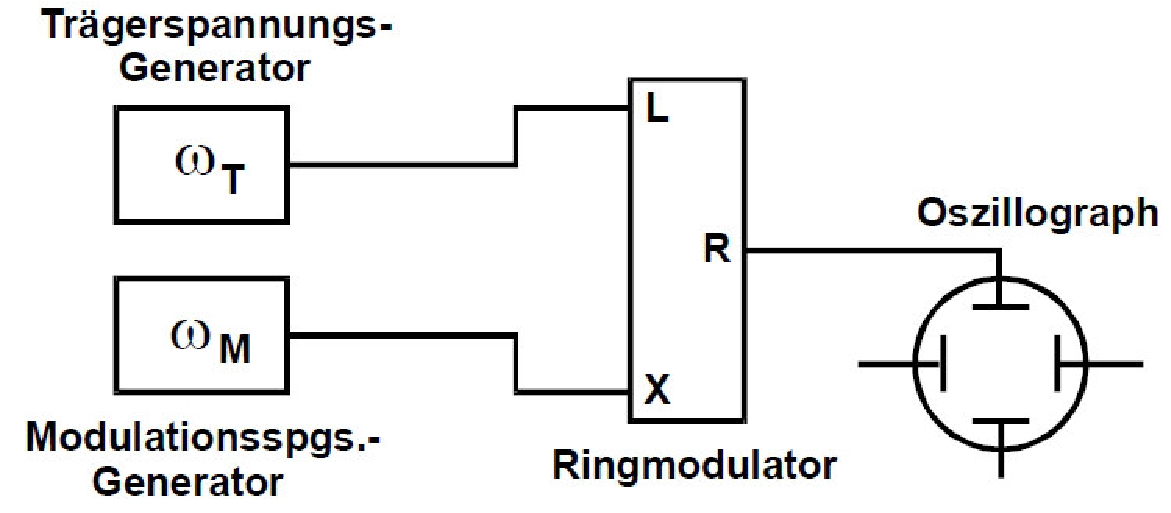
\includegraphics[width = 0.75\textwidth]{../Grafiken/Versuchsaufbau_a.pdf}
	\caption{Die Schaltung mit der die Schwingung einer Amplituden modellierten Spannung aufgenommen wird.\cite{V59}\label{fig:Aufbau_a}}
\end{figure}
Um den Zeitlichen Spannungsverlauf einer amplitudenmodulierten Spannung aufzunehmen wird die Schaltung nach \cref{fig:Aufbau_a} verwendet.
Dabei wird der Spannungsgenerator für die Trägerspannung auf MHz und der für die Modulationsspannung auf kHz.
Dabei wird mithilfe eines Oszilloskop die zeitliche Änderung einer durch einen Ringmodulator erzeugten modulierten Spannung aufgenommen.
Das Frequenzspektrum wird aufgenommen, in dem in \cref{fig:Aufbau_a} das Oszilloskop durch ein Frequenzanalyser ersetzt wird.
Weiter wird einmal die Amplitude mithilfe einer Diode amplitudenmoduliert.

\newpage
\subsection{Demodulation einer Amplitudenmodulierten Spannung}
\begin{figure}[h!]
	\centering
	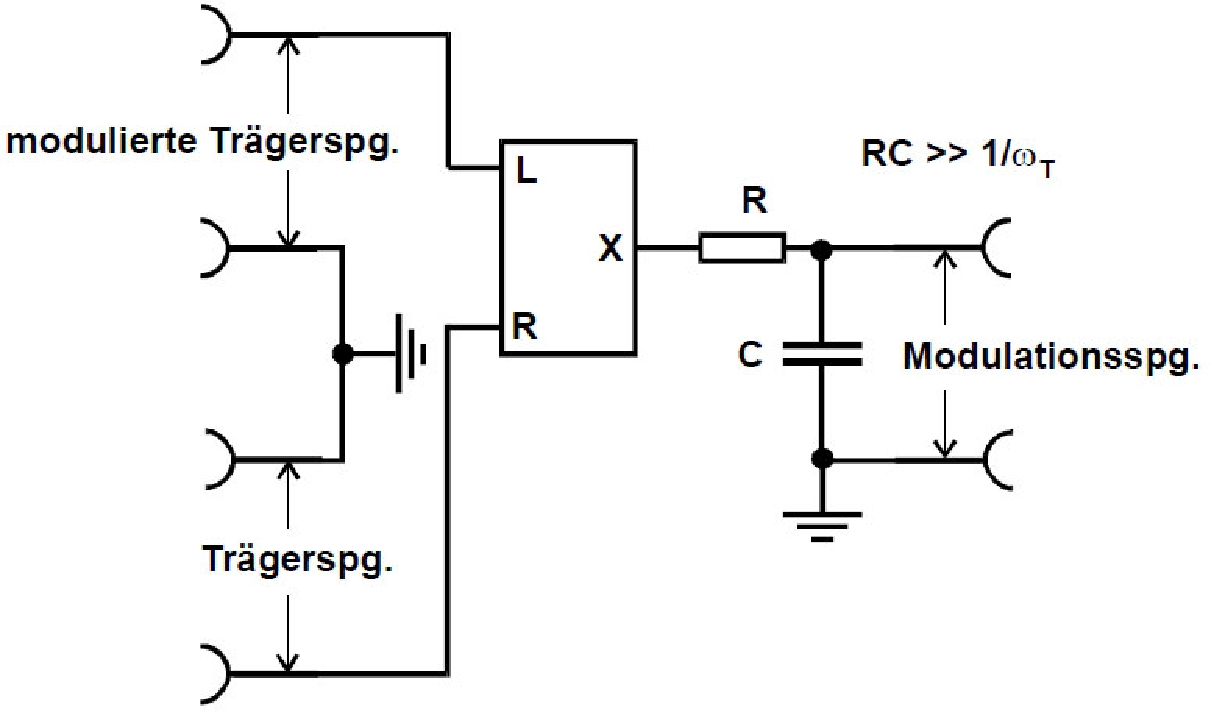
\includegraphics[width = 0.75\textwidth]{../Grafiken/Versuchsaufbau_DemAmplitude_Ringmodulator.pdf}
	\caption{Schaltung für die Demudulation einer Amplitudenmodulierten Spannung.\cite{V59}}
\end{figure}
Die Spannung wird moduliert wie zuvor, mit einem Ringmodulator. 
Dabei wird an die modulierte Trägerspannung an den Eingang L eines Ringmodulators angeschlossen und an Eingang R die unmodulierte Trägerspannung angeschlossen.
An den Ausgang wird ein Tiefpass angeschlossen an dem ein Oszilloskop angeschlossen ist.
Auf dem Zweiten Kanal wird die Modulationsspannung aufgenommen.\\
Weiter wird durch einen Ringmodulator (1) amplitudenmodulierte Spannung demoduliert, unter Verwendung einer Diode (2) und eines Tiefpasses (3).
\begin{figure}[h!]
	\centering
	%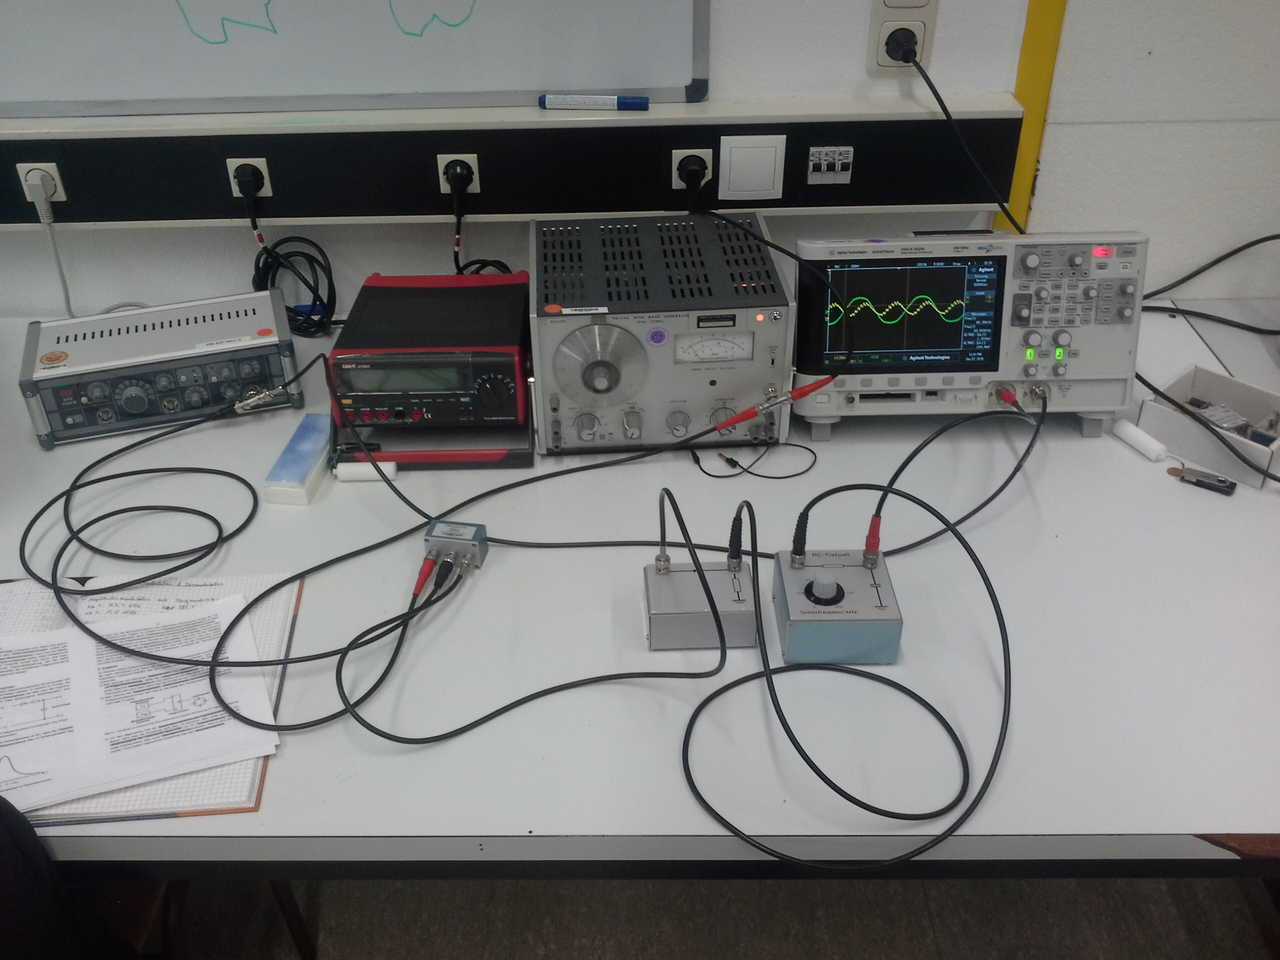
\includegraphics[width = \textwidth/2]{../Grafiken/Versuchsaufbau_g_DemodulationDiode.jpg}
			\begin{tikzpicture}
				\node [draw=white, anchor=south west] (label) at (0,0) {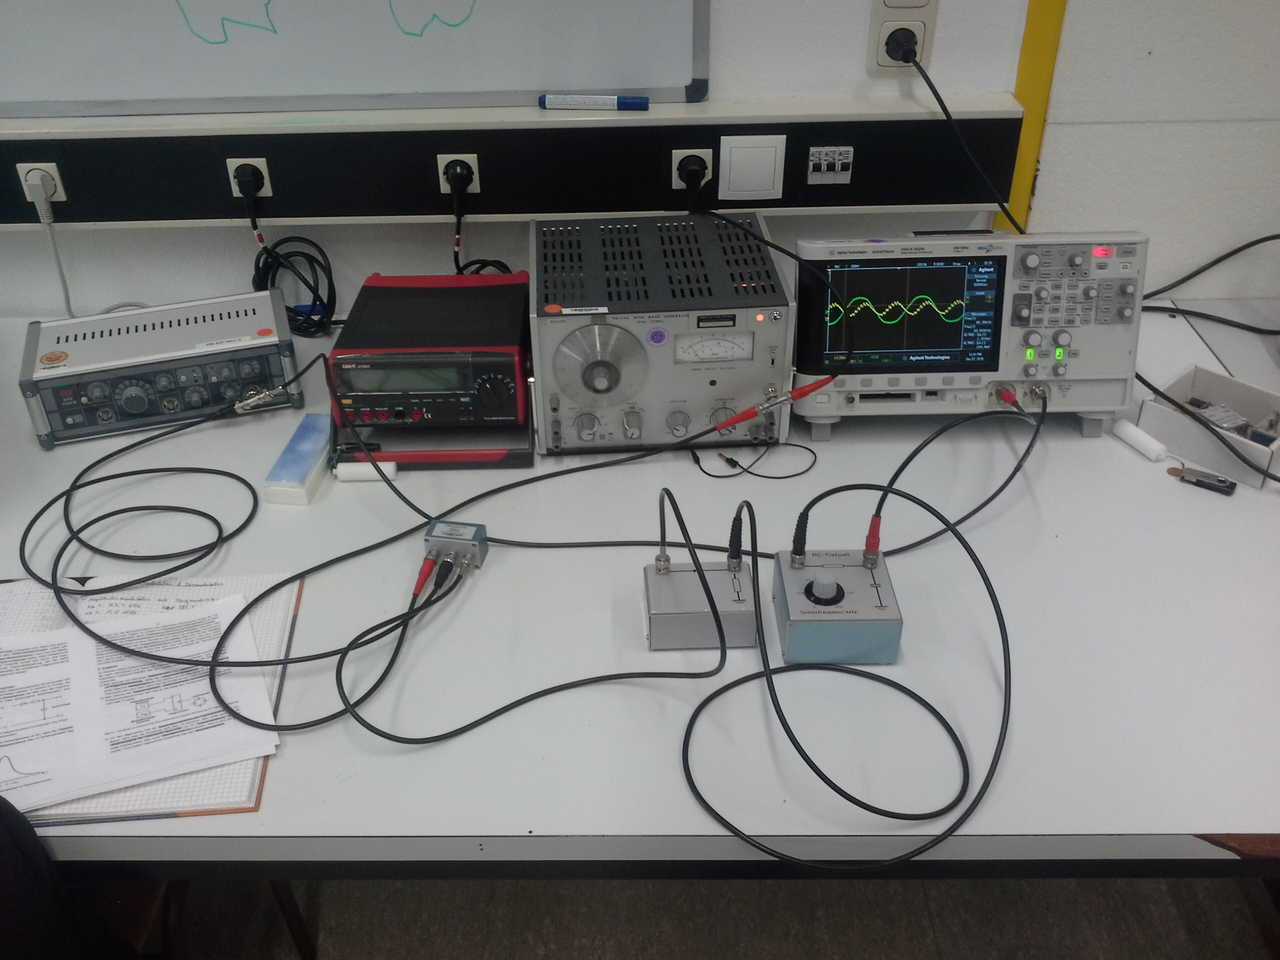
\includegraphics[trim = 0mm 50mm 10mm 70mm , clip ,width = 0.75\textwidth]{../Grafiken/Versuchsaufbau_g_DemodulationDiode.jpg}};
				
				\fill[gray!60!white](3.8,3) circle (0.4);
				\draw(3.8,3) circle (0.4);
				\node at (3.8,3) {$\boldsymbol 1$};

				\fill[gray!60!white](6,2.5) circle (0.4);
				\draw(6,2.5) circle (0.4);
				\node at ( 6,2.5) {$\boldsymbol 2$};
				
				\fill[gray!60!white](9,2.5) circle (0.4);
				\draw(9,2.5) circle (0.4);
				\node at (9,2.5) {$\boldsymbol 2$};
			
			\end{tikzpicture}
	\caption{Schaltung für die Demodulation mithilfe einer Diode und einem Tiefpass.\cite{V59}}
\end{figure}
\newpage
\subsection{Modulation mithilfe einer Diode}
\begin{figure}[h!]
	\centering
	%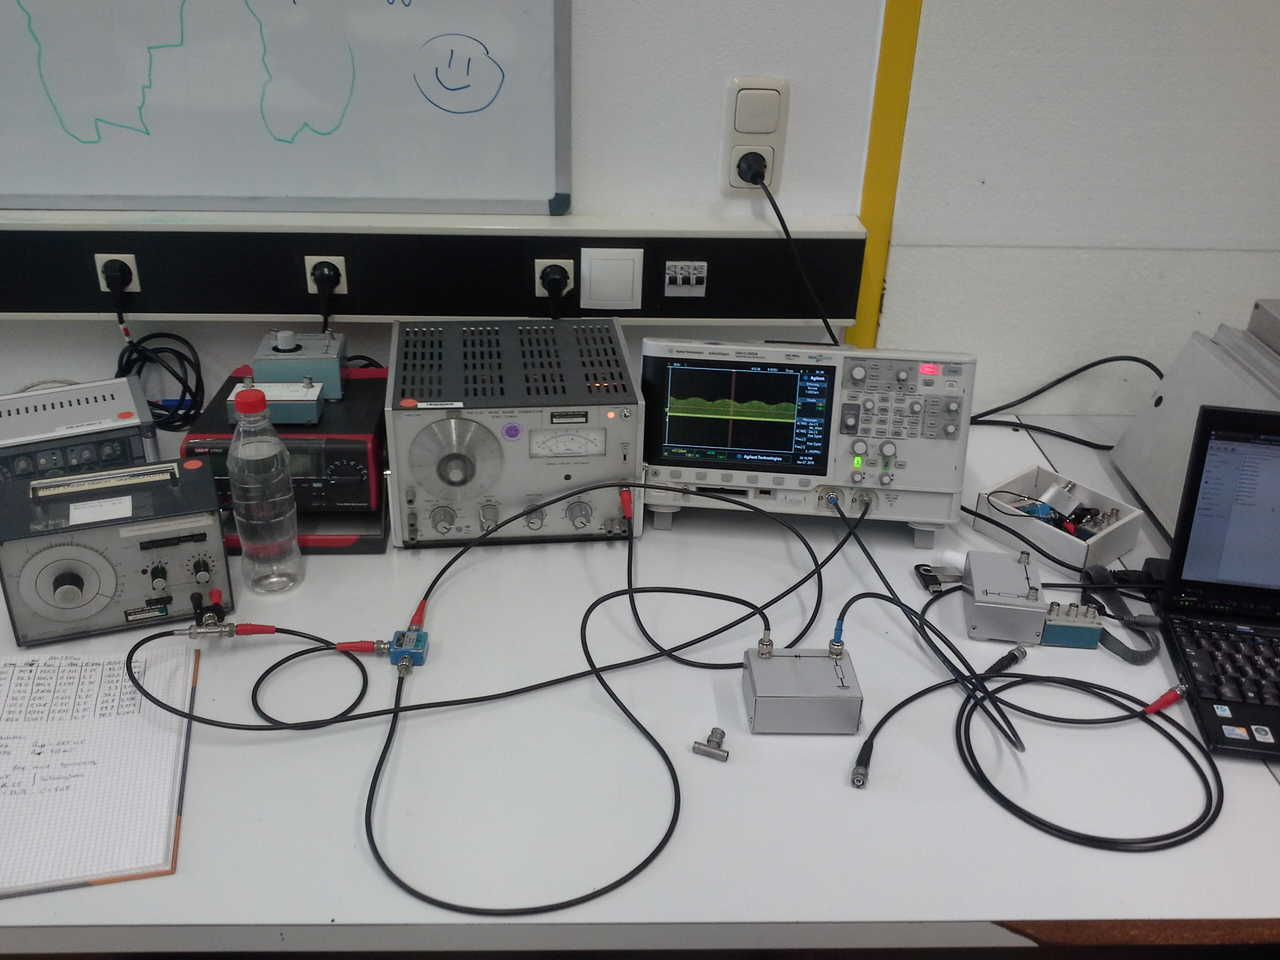
\includegraphics[trim = 10mm 20mm 10mm 100mm , clip ,width = 0.75\textwidth]{../Grafiken/Versuchsaufbau_c_AmpModuliertTraeger.jpg}
			\begin{tikzpicture}
				\node [draw=white, anchor=south west] (label) at (0,0) {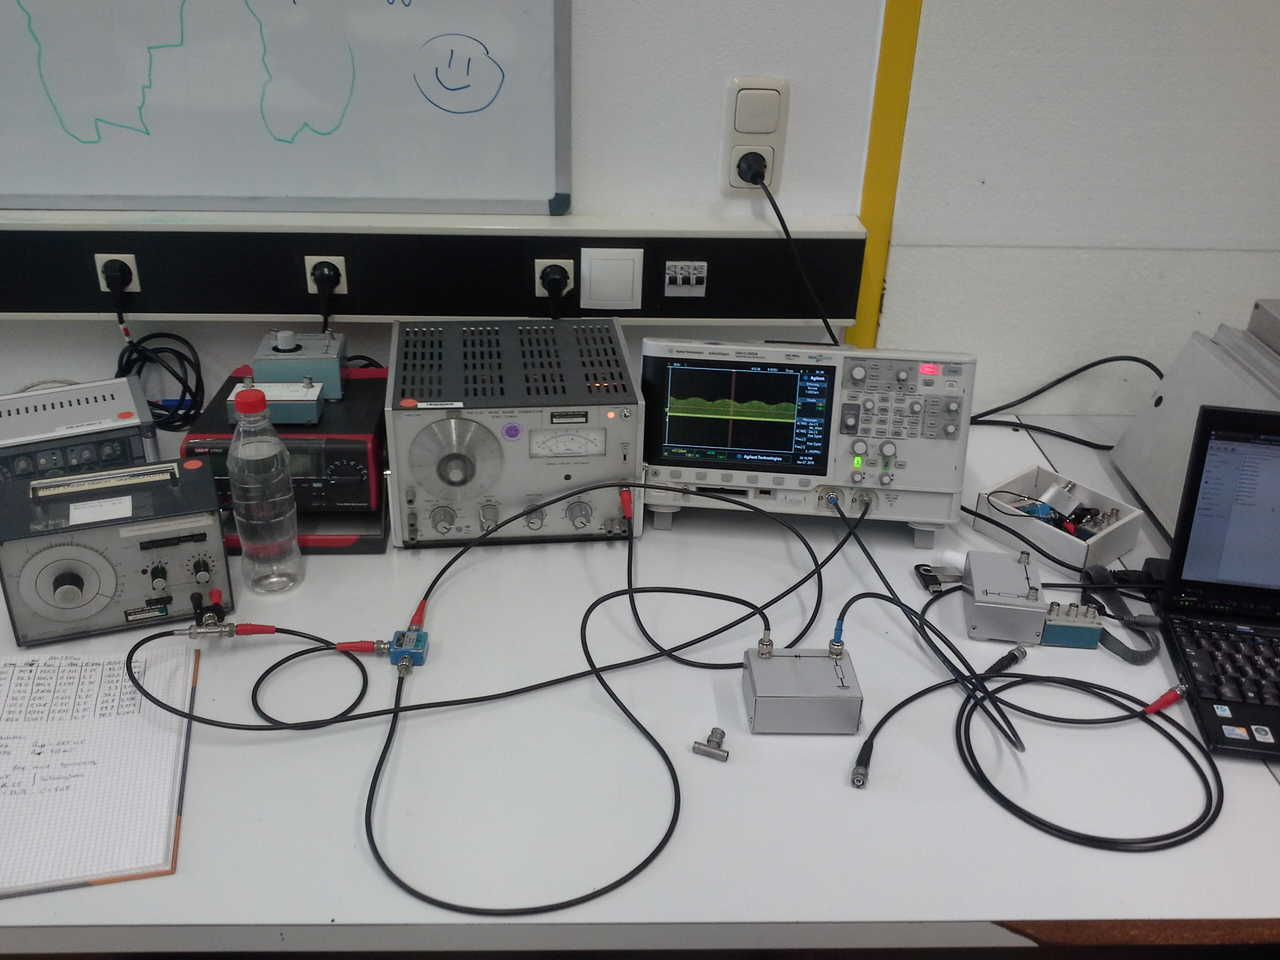
\includegraphics[trim = 0mm 40mm 70mm 100mm , clip ,width = 0.75\textwidth]{../Grafiken/Versuchsaufbau_c_AmpModuliertTraeger.jpg}};
				
				\fill[gray!60!white](1,4) circle (0.4);
				\draw(1,4) circle (0.4);
				\node at (1,4) {$\boldsymbol 1$};
				
				\fill[gray!60!white](5,5.5) circle (0.4);
				\draw(5,5.5) circle (0.4);
				\node at (5,5.5) {$\boldsymbol 2$};
				
				\fill[gray!60!white](10,5.5) circle (0.4);
				\draw(10,5.5) circle (0.4);
				\node at (10,5.5) {$\boldsymbol 4$};
				
				\fill[gray!60!white](10,2) circle (0.4);
				\draw(10,2) circle (0.4);
				\node at (10,2) {$\boldsymbol 3$};
			\end{tikzpicture}
			\caption{Der verwendete Versuchsaufbau für Amplitudenmodulation mit Trägerabstrahlung.}
\end{figure}
Eine Amplitudenmodulation mit Trägerabstrahlung wird erzeugt, mithilfe einer Diode. 
Dabei werden die Generatoren für die Trägerspannung (2) und für die Modulationsspannung (1) in reihe geschaltet mit der Diode (3).
Es wird sowohl die modulierte als auch die Modulationsspannung auf einem Oszilloskop (4) dargestellt.
Für die Modulationsspannung wurde ein batteriebetriebenes Gerät verwendet.
\subsection{Phasenabhängigkeit der Demodulierten Schwingung}
\begin{figure}[h!]
	\centering
	%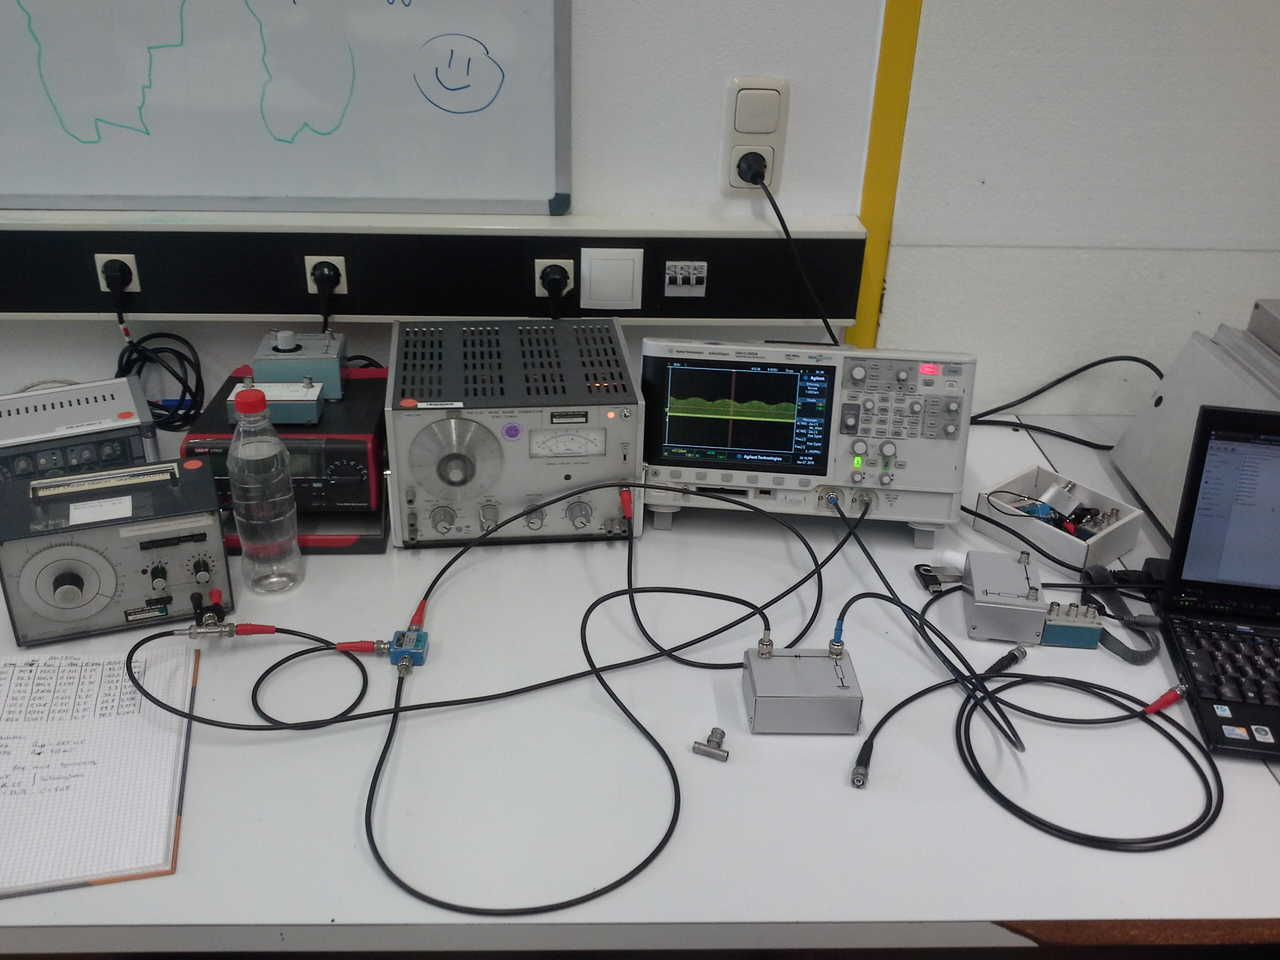
\includegraphics[trim = 10mm 20mm 10mm 100mm , clip ,width = 0.75\textwidth]{../Grafiken/Versuchsaufbau_c_AmpModuliertTraeger.jpg}
			\begin{tikzpicture}
				\node [draw=white, anchor=south west] (label) at (0,0) {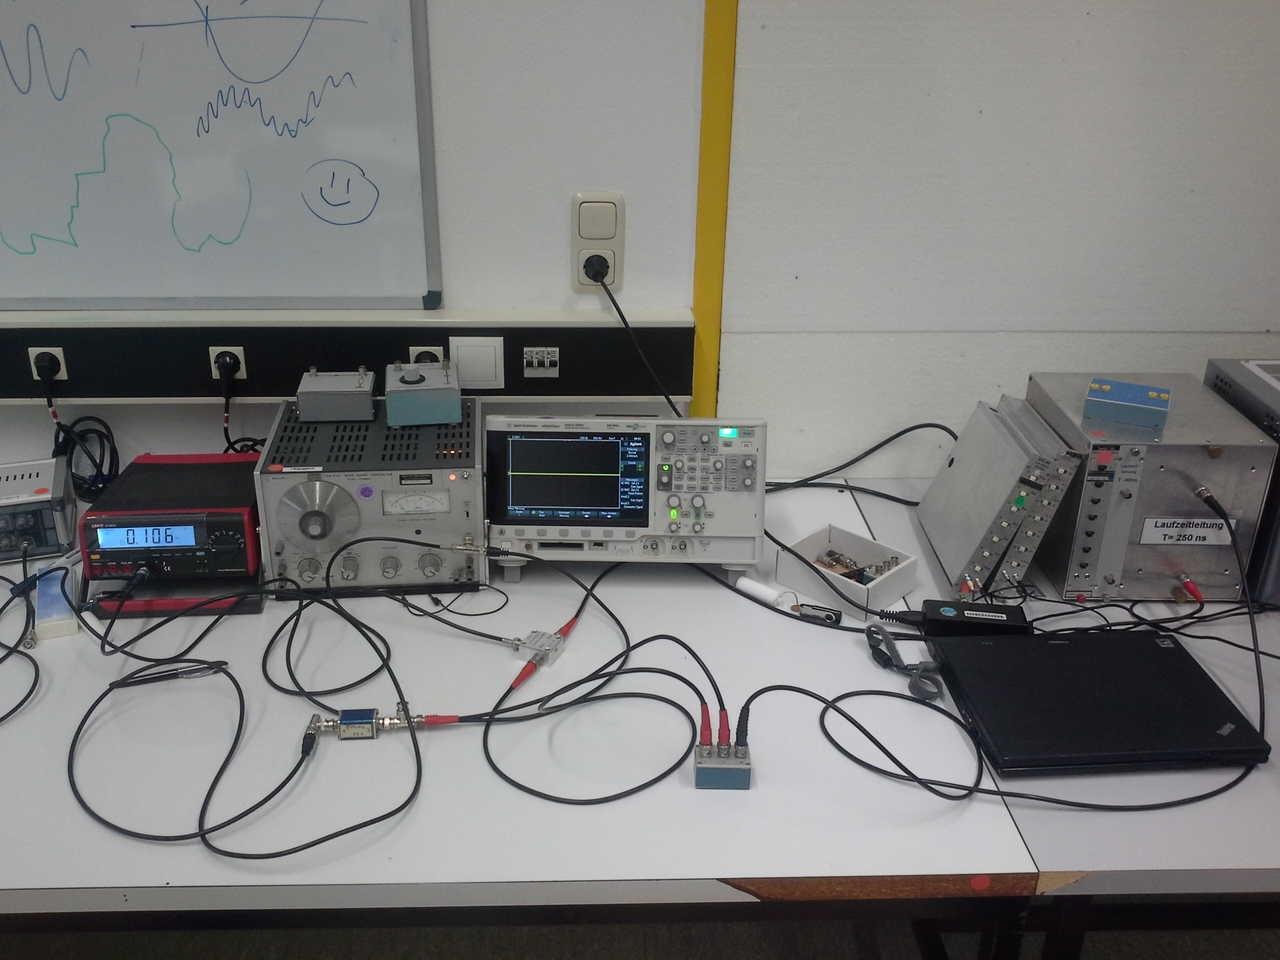
\includegraphics[trim = 20mm 50mm 0mm 130mm , clip ,width = 0.75\textwidth]{../Grafiken/Versuchsaufbau_e_PhasenempfindlicherGleichrichter.jpg}};
				
				\fill[gray!65!white](1,3.5) circle (0.4);
				\draw(1,3.5) circle (0.4);
				\node at (1,3.5) {$\boldsymbol 1$};
				
				\fill[gray!65!white](3,4) circle (0.4);
				\draw(3,4) circle (0.4);
				\node at (3,4) {$\boldsymbol 2$};
				
				\fill[gray!65!white](3.6,1.5) circle (0.4);
				\draw(3.6,1.5) circle (0.4);
				\node at (3.6,1.5) {$\boldsymbol 4$};
				
				\fill[gray!65!white](7.4,1.) circle (0.4);
				\draw(7.4,1.) circle (0.4);
				\node at (7.4,1.) {$\boldsymbol 3$};
				
				\fill[gray!65!white](11,4) circle (0.4);
				\draw(11,4) circle (0.4);
				\node at (11,4) {$\boldsymbol 5$};
			\end{tikzpicture}
			\caption{Der verwendete Versuchsaufbau für die Untersuchung der Phasenabhängigkeit von Modulations- und Trägerspannung.}
\end{figure}
Um die Phasenabhängigkeit der demodulierten Schwingung zu untersuchen, wird ein Hochfrequenzgenerator (2) an beide Eingänge L und R des Ringmodulators (3) angeschlossen, wobei zwischen dem Generator und dem Eingang R ein Phasenschieber (5) geschaltet wird.
Am Ausgang X  wird über einen Tiefpass (4) ein Millivoltmeter (1) angeschlossen.
Hier wird die Spannung in Abhängigkeit der Phasenverstimmung gemessen.
\subsection{Frequenzmodulation}
\begin{figure}[h!]
	\centering
	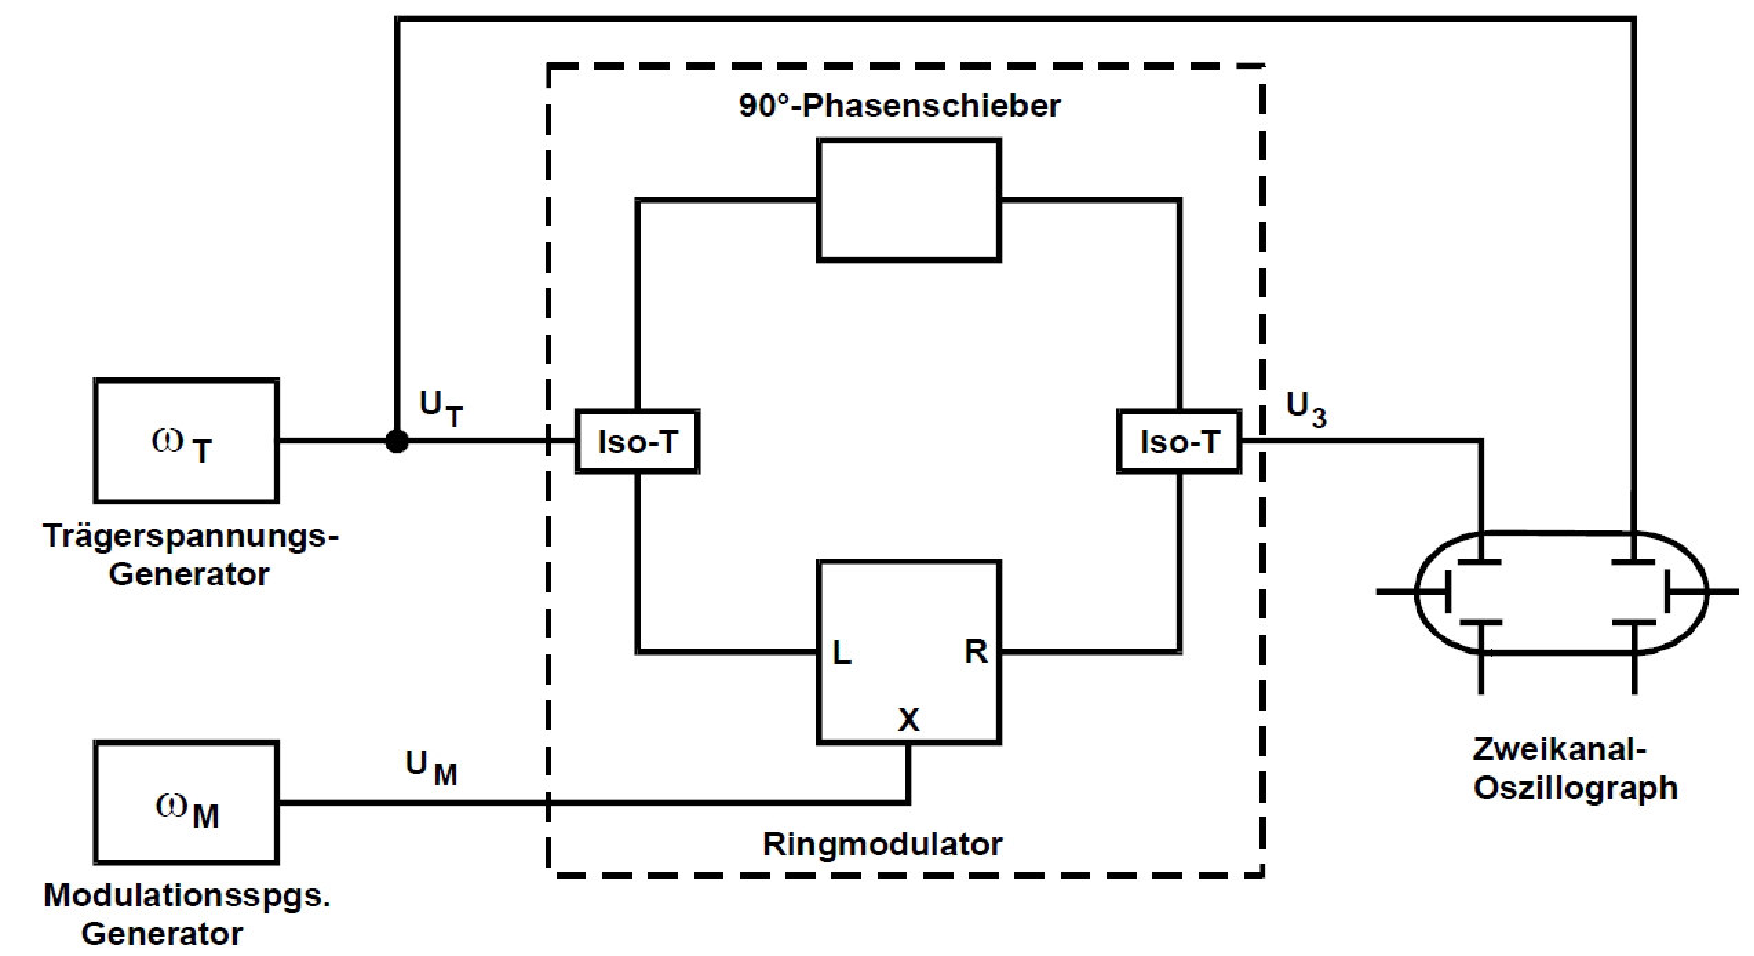
\includegraphics[width = 3\textwidth/4]{../Grafiken/Versuchsaufbau_d_Frequenz.pdf}
	\caption{Die Schaltung für die Frequenzmodulation.\cite{V59}}
\end{figure}
Es wird eine Frequenzmodulation mithilfe eines $90^\circ$-Phasenschieber durch geführt.
Die zeitliche Änderung der modellierten Spannung wird auf einem Oszilloskop sichtbar gemacht, wobei keine Darstellung einer einzelnen Durchlaufs aufgenommen wird.
Auf den zweiten Kanal des Oszilloskops kann die Trägerspannung dargestellt werden.
Weiter wird das Frequenzspektrum der modulierten Schwingung aufgenommen. 
Dies geschieht in dem das Oszilloskop durch einen Frequenzanalyser ausgetauscht wird.
\subsection{Demodulation einer frequenzmodulierten Schwingung}
\begin{figure}[h!]
	\centering
	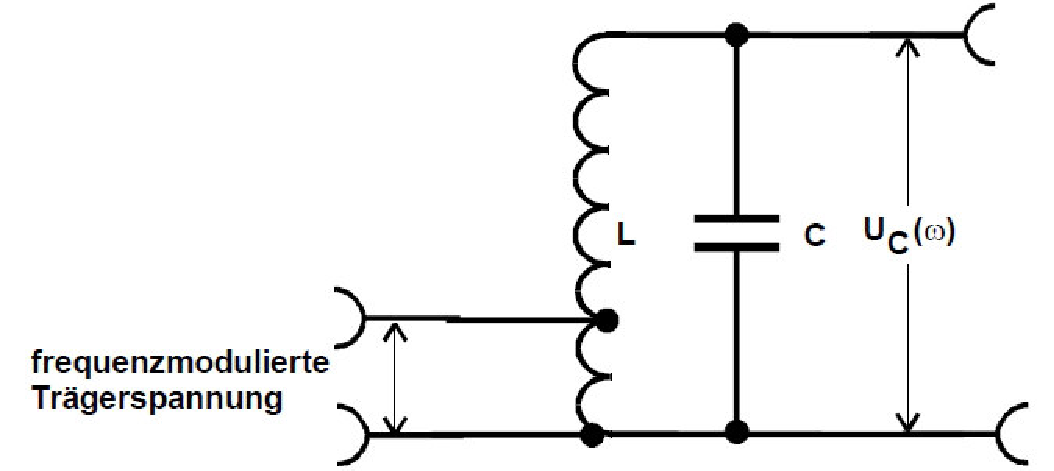
\includegraphics[width = 0.5\textwidth]{../Grafiken/Versuchsaufbau_h_FreqDemo.pdf}
	\caption{Schaltung für eine Demodulation einer Frequenzmodulierten Schwingung.\cite{V59}}
\end{figure}
Die Frequenzmodulierte Schwingung wird mithilfe eines LC-Schwingkreises demoduliert und stellt sie gegen die die Modulationsspannung gegenüber.